%!TEX TS-program = xelatex

\documentclass {article}

\usepackage{xetexko}
\usepackage[a4paper]{geometry}
\usepackage[usenames,dvipsnames]{xcolor}
\usepackage{mathtools}
\usepackage{amsmath}
\usepackage{fontspec}
\usepackage{hyperref}
\usepackage{graphicx}
\usepackage{listings}
\usepackage{makeidx}
\usepackage{indentfirst}
\usepackage{tikz}
\usetikzlibrary{arrows,automata}


%\setmainfont {NanumMyeongjo}
\setmainfont {UnBatang}
\setmonofont[Scale=0.8]{DejaVu Sans Mono}

\lstdefinestyle{diff}{
  belowcaptionskip=1\baselineskip,
  breaklines=true,
  frame=L,
  xleftmargin=\parindent,
  showstringspaces=false,
  % Diffstart
  morecomment=[f][\color{gray}]{@@},
  % Diffincl
  morecomment=[f][\color{Green}]{+},
  % Diffrem
  morecomment=[f][\color{Red}]{-},
  basicstyle=\footnotesize\ttfamily,
}

\lstdefinestyle{customtxt}{
  belowcaptionskip=1\baselineskip,
  breaklines=true,
  frame=L,
  xleftmargin=\parindent,
  showstringspaces=false,
  basicstyle=\footnotesize\ttfamily,
}

\lstdefinestyle{customc}{
  belowcaptionskip=1\baselineskip,
  breaklines=true,
  frame=L,
  xleftmargin=\parindent,
  language=C,
  showstringspaces=false,
  basicstyle=\footnotesize\ttfamily,
  keywordstyle=\bfseries\color{green!40!black},
  commentstyle=\itshape\color{purple!40!black},
  identifierstyle=\color{blue},
  stringstyle=\color{orange},
}

\lstdefinestyle{customrs}{
  belowcaptionskip=1\baselineskip,
  breaklines=true,
  frame=L,
  xleftmargin=\parindent,
  showstringspaces=false,
  morekeywords={fn,let,mut,pub,use,impl,struct,unsafe,if,for},
  morecomment=[l]{//},
  morecomment=[n]{/*}{*/},
  basicstyle=\footnotesize\ttfamily,
  keywordstyle=\bfseries\color{green!40!black},
  commentstyle=\itshape\color{purple!40!black},
  identifierstyle=\color{blue},
  stringstyle=\color{orange},
}


\begin {document}

\title {Ext3 과 NILFS2 의 Block I/O 패턴 비교}
\input {../../reportauthor.tex}
\maketitle

\section{Ext3 과 NILFS2 의 비교}
Ext3 파일 시스템은 저널링 파일 시스템이다. Ext3 은 기본적으로 저널에 메타정보와 파일 내용을 기록 후, 이를 디스크 영역에 적어넣는다. 반면,
NILFS2 파일 시스템은 Log-structed 파일 시스템이다. 이는 로그를 연속된 블럭으로 저장하는 방식으로 데이터를 적어넣는다.

이 두 파일 시스템의 차이가 만들어내는 Block write 패턴은, 아래의 벤치마크 결과에서 Block I/O 패턴의 차이로 나타나게 된다.
\section{Block I/O 결과}
\subsection{사용된 환경}
\setlength{\parindent}{0cm}
툴체인
\begin{lstlisting}[style=customtxt]
  arm-eabi-4.6 from Android Open-source Project
\end{lstlisting}
원본 커널 소스 코드 리버전
\begin{lstlisting}[style=customtxt]
Tizen TRATS2 kernel code commit c349d3966a91b3036d9e4a16a7849ab23d1e6435
(branch tizen_2.3, retrieved from Tizen gerrit code review, identical as TA version)
\end{lstlisting}
iozone 옵션
\begin{lstlisting}[style=customtxt]
  iozone -a -i 0 -n 32m -g 32m -r 16k
\end{lstlisting}
FS image size: 각각 256MiB
\newpage
\subsection{결과}
\subsubsection{Ext3}
\begin{figure} [h!]
    \caption{ext3}
    \begin{center}
      \resizebox{0.5\textwidth}{!}{
        % GNUPLOT: LaTeX picture with Postscript
\begingroup
  \makeatletter
  \providecommand\color[2][]{%
    \GenericError{(gnuplot) \space\space\space\@spaces}{%
      Package color not loaded in conjunction with
      terminal option `colourtext'%
    }{See the gnuplot documentation for explanation.%
    }{Either use 'blacktext' in gnuplot or load the package
      color.sty in LaTeX.}%
    \renewcommand\color[2][]{}%
  }%
  \providecommand\includegraphics[2][]{%
    \GenericError{(gnuplot) \space\space\space\@spaces}{%
      Package graphicx or graphics not loaded%
    }{See the gnuplot documentation for explanation.%
    }{The gnuplot epslatex terminal needs graphicx.sty or graphics.sty.}%
    \renewcommand\includegraphics[2][]{}%
  }%
  \providecommand\rotatebox[2]{#2}%
  \@ifundefined{ifGPcolor}{%
    \newif\ifGPcolor
    \GPcolorfalse
  }{}%
  \@ifundefined{ifGPblacktext}{%
    \newif\ifGPblacktext
    \GPblacktexttrue
  }{}%
  % define a \g@addto@macro without @ in the name:
  \let\gplgaddtomacro\g@addto@macro
  % define empty templates for all commands taking text:
  \gdef\gplbacktext{}%
  \gdef\gplfronttext{}%
  \makeatother
  \ifGPblacktext
    % no textcolor at all
    \def\colorrgb#1{}%
    \def\colorgray#1{}%
  \else
    % gray or color?
    \ifGPcolor
      \def\colorrgb#1{\color[rgb]{#1}}%
      \def\colorgray#1{\color[gray]{#1}}%
      \expandafter\def\csname LTw\endcsname{\color{white}}%
      \expandafter\def\csname LTb\endcsname{\color{black}}%
      \expandafter\def\csname LTa\endcsname{\color{black}}%
      \expandafter\def\csname LT0\endcsname{\color[rgb]{1,0,0}}%
      \expandafter\def\csname LT1\endcsname{\color[rgb]{0,1,0}}%
      \expandafter\def\csname LT2\endcsname{\color[rgb]{0,0,1}}%
      \expandafter\def\csname LT3\endcsname{\color[rgb]{1,0,1}}%
      \expandafter\def\csname LT4\endcsname{\color[rgb]{0,1,1}}%
      \expandafter\def\csname LT5\endcsname{\color[rgb]{1,1,0}}%
      \expandafter\def\csname LT6\endcsname{\color[rgb]{0,0,0}}%
      \expandafter\def\csname LT7\endcsname{\color[rgb]{1,0.3,0}}%
      \expandafter\def\csname LT8\endcsname{\color[rgb]{0.5,0.5,0.5}}%
    \else
      % gray
      \def\colorrgb#1{\color{black}}%
      \def\colorgray#1{\color[gray]{#1}}%
      \expandafter\def\csname LTw\endcsname{\color{white}}%
      \expandafter\def\csname LTb\endcsname{\color{black}}%
      \expandafter\def\csname LTa\endcsname{\color{black}}%
      \expandafter\def\csname LT0\endcsname{\color{black}}%
      \expandafter\def\csname LT1\endcsname{\color{black}}%
      \expandafter\def\csname LT2\endcsname{\color{black}}%
      \expandafter\def\csname LT3\endcsname{\color{black}}%
      \expandafter\def\csname LT4\endcsname{\color{black}}%
      \expandafter\def\csname LT5\endcsname{\color{black}}%
      \expandafter\def\csname LT6\endcsname{\color{black}}%
      \expandafter\def\csname LT7\endcsname{\color{black}}%
      \expandafter\def\csname LT8\endcsname{\color{black}}%
    \fi
  \fi
  \setlength{\unitlength}{0.0500bp}%
  \begin{picture}(7200.00,5040.00)%
    \gplgaddtomacro\gplbacktext{%
      \csname LTb\endcsname%
      \put(1122,440){\makebox(0,0)[r]{\strut{} 0}}%
      \put(1122,1163){\makebox(0,0)[r]{\strut{} 20000}}%
      \put(1122,1885){\makebox(0,0)[r]{\strut{} 40000}}%
      \put(1122,2608){\makebox(0,0)[r]{\strut{} 60000}}%
      \put(1122,3330){\makebox(0,0)[r]{\strut{} 80000}}%
      \put(1122,4052){\makebox(0,0)[r]{\strut{} 100000}}%
      \put(1122,4775){\makebox(0,0)[r]{\strut{} 120000}}%
      \put(1254,220){\makebox(0,0){\strut{} 0}}%
      \put(2047,220){\makebox(0,0){\strut{} 5000}}%
      \put(2839,220){\makebox(0,0){\strut{} 10000}}%
      \put(3632,220){\makebox(0,0){\strut{} 15000}}%
      \put(4425,220){\makebox(0,0){\strut{} 20000}}%
      \put(5218,220){\makebox(0,0){\strut{} 25000}}%
      \put(6010,220){\makebox(0,0){\strut{} 30000}}%
      \put(6803,220){\makebox(0,0){\strut{} 35000}}%
    }%
    \gplgaddtomacro\gplfronttext{%
    }%
    \gplbacktext
    \put(0,0){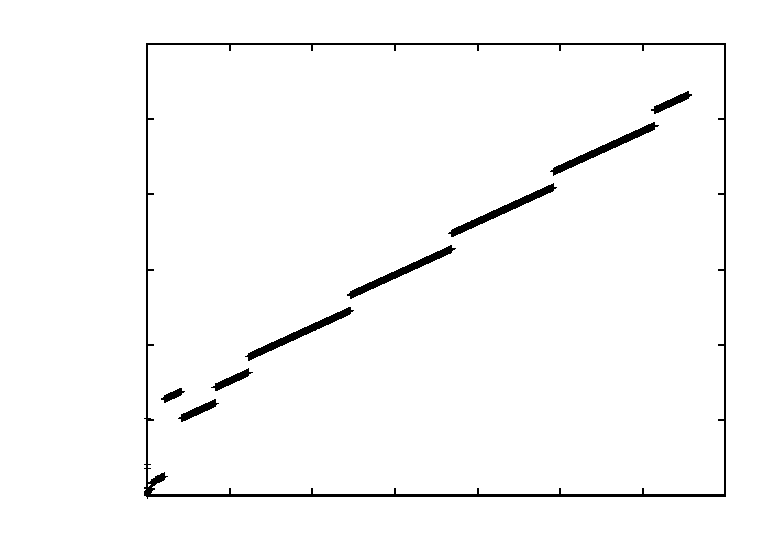
\includegraphics{iozone_ext3}}%
    \gplfronttext
  \end{picture}%
\endgroup

      }
    \end{center}
\end{figure}
Ext3 의 경우, 저널링 파일 시스템의 특성을 Block I/O 결과에서 나타내고 있다. 블럭에 쓰기를 할 때, 2블럭씩 저널에 쓴 뒤, 이를 실제 디스크 영역에 작성하게 된다.

따라서, 파일 쓰기 그래프가 순차적으로 쓰여지지 않고, 끊어지게 된다.
\subsubsection{NILFS2}
\begin{figure} [h!]
  \caption{nilfs2}
  \begin{center}
    \resizebox{0.5\textwidth}{!}{
      % GNUPLOT: LaTeX picture with Postscript
\begingroup
  \makeatletter
  \providecommand\color[2][]{%
    \GenericError{(gnuplot) \space\space\space\@spaces}{%
      Package color not loaded in conjunction with
      terminal option `colourtext'%
    }{See the gnuplot documentation for explanation.%
    }{Either use 'blacktext' in gnuplot or load the package
      color.sty in LaTeX.}%
    \renewcommand\color[2][]{}%
  }%
  \providecommand\includegraphics[2][]{%
    \GenericError{(gnuplot) \space\space\space\@spaces}{%
      Package graphicx or graphics not loaded%
    }{See the gnuplot documentation for explanation.%
    }{The gnuplot epslatex terminal needs graphicx.sty or graphics.sty.}%
    \renewcommand\includegraphics[2][]{}%
  }%
  \providecommand\rotatebox[2]{#2}%
  \@ifundefined{ifGPcolor}{%
    \newif\ifGPcolor
    \GPcolorfalse
  }{}%
  \@ifundefined{ifGPblacktext}{%
    \newif\ifGPblacktext
    \GPblacktexttrue
  }{}%
  % define a \g@addto@macro without @ in the name:
  \let\gplgaddtomacro\g@addto@macro
  % define empty templates for all commands taking text:
  \gdef\gplbacktext{}%
  \gdef\gplfronttext{}%
  \makeatother
  \ifGPblacktext
    % no textcolor at all
    \def\colorrgb#1{}%
    \def\colorgray#1{}%
  \else
    % gray or color?
    \ifGPcolor
      \def\colorrgb#1{\color[rgb]{#1}}%
      \def\colorgray#1{\color[gray]{#1}}%
      \expandafter\def\csname LTw\endcsname{\color{white}}%
      \expandafter\def\csname LTb\endcsname{\color{black}}%
      \expandafter\def\csname LTa\endcsname{\color{black}}%
      \expandafter\def\csname LT0\endcsname{\color[rgb]{1,0,0}}%
      \expandafter\def\csname LT1\endcsname{\color[rgb]{0,1,0}}%
      \expandafter\def\csname LT2\endcsname{\color[rgb]{0,0,1}}%
      \expandafter\def\csname LT3\endcsname{\color[rgb]{1,0,1}}%
      \expandafter\def\csname LT4\endcsname{\color[rgb]{0,1,1}}%
      \expandafter\def\csname LT5\endcsname{\color[rgb]{1,1,0}}%
      \expandafter\def\csname LT6\endcsname{\color[rgb]{0,0,0}}%
      \expandafter\def\csname LT7\endcsname{\color[rgb]{1,0.3,0}}%
      \expandafter\def\csname LT8\endcsname{\color[rgb]{0.5,0.5,0.5}}%
    \else
      % gray
      \def\colorrgb#1{\color{black}}%
      \def\colorgray#1{\color[gray]{#1}}%
      \expandafter\def\csname LTw\endcsname{\color{white}}%
      \expandafter\def\csname LTb\endcsname{\color{black}}%
      \expandafter\def\csname LTa\endcsname{\color{black}}%
      \expandafter\def\csname LT0\endcsname{\color{black}}%
      \expandafter\def\csname LT1\endcsname{\color{black}}%
      \expandafter\def\csname LT2\endcsname{\color{black}}%
      \expandafter\def\csname LT3\endcsname{\color{black}}%
      \expandafter\def\csname LT4\endcsname{\color{black}}%
      \expandafter\def\csname LT5\endcsname{\color{black}}%
      \expandafter\def\csname LT6\endcsname{\color{black}}%
      \expandafter\def\csname LT7\endcsname{\color{black}}%
      \expandafter\def\csname LT8\endcsname{\color{black}}%
    \fi
  \fi
  \setlength{\unitlength}{0.0500bp}%
  \begin{picture}(7200.00,5040.00)%
    \gplgaddtomacro\gplbacktext{%
      \csname LTb\endcsname%
      \put(1122,440){\makebox(0,0)[r]{\strut{} 0}}%
      \put(1122,1018){\makebox(0,0)[r]{\strut{} 20000}}%
      \put(1122,1596){\makebox(0,0)[r]{\strut{} 40000}}%
      \put(1122,2174){\makebox(0,0)[r]{\strut{} 60000}}%
      \put(1122,2752){\makebox(0,0)[r]{\strut{} 80000}}%
      \put(1122,3330){\makebox(0,0)[r]{\strut{} 100000}}%
      \put(1122,3908){\makebox(0,0)[r]{\strut{} 120000}}%
      \put(1122,4486){\makebox(0,0)[r]{\strut{} 140000}}%
      \put(1254,220){\makebox(0,0){\strut{} 0}}%
      \put(2179,220){\makebox(0,0){\strut{} 100}}%
      \put(3104,220){\makebox(0,0){\strut{} 200}}%
      \put(4029,220){\makebox(0,0){\strut{} 300}}%
      \put(4953,220){\makebox(0,0){\strut{} 400}}%
      \put(5878,220){\makebox(0,0){\strut{} 500}}%
      \put(6803,220){\makebox(0,0){\strut{} 600}}%
    }%
    \gplgaddtomacro\gplfronttext{%
    }%
    \gplbacktext
    \put(0,0){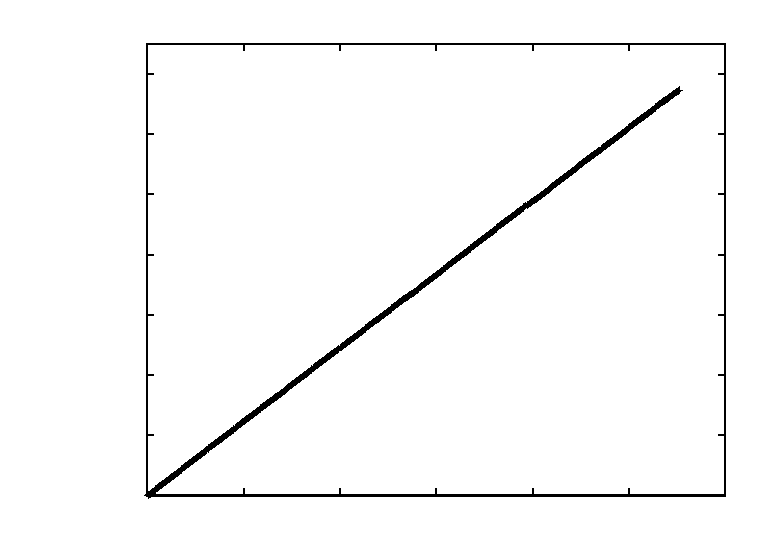
\includegraphics{iozone_nilfs2}}%
    \gplfronttext
  \end{picture}%
\endgroup

    }
  \end{center}
\end{figure}
NILFS2 의 경우, Log-structed 파일 시스템의 특성을 나타내고 있다. NILFS write 의 경우, segctord 데몬이, 쓰기 요청을 모아, 약 248블럭씩 로그에 지속적으로 작성하는 것을 볼 수 있다.

이는 Ext3 의 Block I/O 패턴과 다르게, 순차적으로 파일이 쓰여지는 패턴을 보이게 된다.

\newpage
\section{부록}
\subsection{소스 코드}
\lstinputlisting [style=customc]{srcs/bio-benchmark.c}
\subsection{Patchset}
\setlength{\parindent}{0cm}
0001-Fix-compile-error-due-to-missing-sys-ioccom.h.-https.patch
\lstinputlisting [style=diff]{patchset/0001-Fix-compile-error-due-to-missing-sys-ioccom.h.-https.patch}
0002-Samsung-s-fallback-does-not-work.-Since-we-does-not-.patch
\lstinputlisting [style=diff]{patchset/0002-Samsung-s-fallback-does-not-work.-Since-we-does-not-.patch}
0003-sudo-without-password-might-be-bad-idea.patch
\lstinputlisting [style=diff]{patchset/0003-sudo-without-password-might-be-bad-idea.patch}
0004-path-fix.patch
\lstinputlisting [style=diff]{patchset/0004-path-fix.patch}
0005-Block-I-O-benchmark-code.patch
\lstinputlisting [style=diff]{patchset/0005-Block-I-O-benchmark-code.patch}
\end {document}
